\documentclass[12pt]{article}
\usepackage[utf8]{inputenc}
\usepackage{graphicx} 
\usepackage{wrapfig}
\usepackage[dvipsnames]{xcolor}
\usepackage{moreverb}
\usepackage{ragged2e}
\renewcommand\refname{Referencias}
\title{Elementos de la programación Python 1.}
\author{\textcolor{JungleGreen}{Olga María Fimbres Morales}}
\date{17 de Enero 2016}
\begin{document}
\begin{titlepage}
\pagecolor{black!85}
\color{white}
\begin{center}
\begin{large}
Universidad del Estado de Sonora\\
\end{large}
\vspace*{0.15in}
División de Ciencias Exactas y Naturales.\\
\vspace*{0.15in}
Licenciatura en Física. \\
\vspace*{0.6in}
\begin{large}
Física Computacional 1\\
\end{large}
\vspace*{0.2in}
\begin{Large}
\Huge{\textbf{{\textcolor{Red}{Apocalipsis Zombie.}}}} \\
\end{Large}

%\begin{Large}
%\textbf{{\textcolor{Red}{Péndulo.}}} \\
%end{Large}
%\vspace*{-1in}

\rule{80mm}{0.1mm}\\
\vspace*{0.1in}
\begin{large}
{Olga María Fimbres Morales}\\
1 de Mayo de 2016\\
\end{large}
\end{center}
\end{titlepage}

\pagebreak
\color{white}
\section*{Introducción.}
 Para finalizar el curso de \textcolor{LimeGreen}{Física Computacional 1} se escogió un modelo de simulación referente al cambio de dos poblaciones que conviven entre ellas, siendo una la depredadora de la otra. Para ilustrar esta situación presentamos el modelo de un \textcolor{Red}{Apocalipsis zombie} para diferentes situaciones en las que este se puede representar.\\
 
 Resulta interesante saber que utilizando las herramientas que durante este curso hemos analizando es posible crear cualquier escenario que se nos ocurra para una simulación y su eventual estudio.\\
 
 Así que, de la misma forma que aquí mostramos y desarrollamos un escenario de fantasía, somos capaces de crear cualquier otro que sea de utilidad para nuestros diferentes proyectos.\\
 
 Mostrando la facilidad que nos brinda el ser capaces de definir un modelo de una forma matemática y además de esto ser capaces de resolverlo y conocer la forma en que este tenderá a comportarse a lo largo de nuestro estudio; o bien nos brinda una idea de las expectativas que debemos tener al momento de desarrollar diferentes experimentos y de esta forma ser capaces de especular un resultado y decidir, incluso antes de comenzar, si nuestra elección de experimento es la correcta para nuestros objetivos.
 
 
 
 
\section*{\textcolor{Red}{Zombies.}}

Los zombies es el termino que se asocia a la persona infectada por un virus, puede ser de diferente tipo, que le provoca que su cerebro deje de funcionar como el de un humano promedio ocasionando con ello un detenimiento de sus sistemas internos , convirtiéndolo de esta forma en un cadáver con la capacidad de moverse.\\ 

Su principal característica es el hecho de que a pesar de no estar vivos poseen una insaciable hambre de carne humana. Siendo de este modo una amenaza para los no infectados.\\

Siendo pocas las posibilidades que poseen los humanos para actuar ante una crisis como esta; se han manejado en la literatura y el cine diferentes planes de acción, como lo es el concentrar a los infectados en una zoma de cuarentena, buscar una cura o simplemente eliminarlos para acabar con la amenaza.\\

Del mismo modo, existen distintos tipos de zombies, algunos de ellos son:

\begin{itemize}
\item Zombie genérico.- Es una persona que tras haber muerto es reanimado a causa de un virus, generalmente son violentos y curiosos.
\item Corredores.- Representan una gran amenaza para los sobrevivientes ya que tienen la capacidad de correr aun en su estado de cadáver; a pesar de tener esta capacidad son poco resistentes y pueden ser eliminador por una herida en el pecho, desangrados o inanición.
\item Stalkers.- Son los zombies más salvajes, de mueven sobre sus cuatro extremidades, posiblemente debido al deterioro de su cerebro que ocasiona una reducción de las capacidades motoras. Llegan incluso a atacar a otros zombies.
\item Bonies.- Es la última etapa de zombificación y ocurre cuando la mayoría de la carne y piel se han desprendido, dejando únicamente huesos y tendones expuestos. A pesar de no tener ojos poseen una ecolocalización que es lo que les permite moverse en su ambiente aunque de una forma lenta si no se encuentran cerca de un humano.
\end{itemize}

Es de conocimiento popular que el mejor m\'etodo para eliminar a un zombie es por medio de la destrucci\'on de su cerebro, lo que deja a los humanos es desventaja por la cercanía que debe de tenerse con el zombie para lograr esto.\\

A lo largo de los años este ha sido un tema recurrente en películas y libros de terror, ganando popularidad en diferentes etapas hasta el punto en que se encuentran incluso dentro del ámbito de la comedia.



\pagebreak
\section*{\textcolor{Red}{Problema.}}

En el desarrollo de la presente práctica se nos proporciona un código base que simula un apocalipsis zombie básica, es decir, que solo toma en cuenta a los humanos que pueden ser convertidos, los zombies y los removidos; siendo por esto mismo pocos los parámetros que afectan a nuestro  modelo:\\

\begin{boxedverbatim}
#Parámetros
P = 0       # Tasa de Natalidad
d = 0.0001  # Muertes naturales por día
B = 0.0095  # Parámetro de transmisión  (per day)
G = 0.0001  # Removidos que se convierten en zombies (per day)
A = 0.0001  # Destruidos  (per day)

# solve the system dy/dt = f(y, t)
def f(y, t):
    Si = y[0] #suceptibles a convertirse
    Zi = y[1] #Zombies
    Ri = y[2] #removidos
    # Sistema de ecuaciones
    f0 = P - B*Si*Zi - d*Si #Suceptibles
    f1 = B*Si*Zi + G*Ri - A*Si*Zi #Zombies
    f2 = d*Si + A*Si*Zi - G*Ri #Removimos
    return [f0, f1, f2]

# Condiciones Iniciales
S0 = 500.                   # Pobación humana
Z0 = 0                      # Población zombie
R0 = 0                      # Población muerta
y0 = [S0, Z0, R0]   # initial condition vector
t  = np.linspace(0, 5., 1000)       # Tiempo

\end{boxedverbatim}\\
\\

Como podemos ver el modelo se describe por medio de una serie de ecuaciones que definen la cantidad de humanos y zombies presentes en el escenario. A partir de este modelo básico es que se nos pide desarrollar los diferentes escenarios, modificando los debidos aspectos para cubrir las posibilidades que nos muestra el nuevo modelo.\\

Cada uno de los casos posee una característica diferente al anterior que queda evidenciado en la forma en que ahora se expresa el modelo; por ejemplo, abordemos el modelo básico, donde el número de personas susceptibles se encuentra definido por una suma de factores que aportan de una forma positiva o negativa compuestos por los diversos parámetros.\\

 \begin{verbatim}
 # Sistema de ecuaciones
    S' = P - B*Si*Zi - d*Si 
    Z' = B*Si*Zi + G*Ri - A*Si*Zi
    R' = d*Si + A*Si*Zi - G*Ri 
 \end{verbatim}

Podemos observar que por ejemplo la población de zombies se encuentra definida por el parámetro de transmisión del virus que afecta a su vez a la población de susceptibles, también se ve aumentada por la cantidad de removidos que son transformados en zombies; pero sin embargo se ve reducida por la cantidad de los que son eliminados.\\

Por otro lado, si analizamos el escenario del modelo donde existe la infección latente entre la población observamos lo siguiente:

\begin{verbatim}
# Sistema de ecuaciones
    S' = P - B*Si*Zi - d*Si 
    Z' = p*Ii + G*Ri - A*Si*Zi 
    R' = d*Si + d*Ii+ A*Si*Zi - G*Ri 
    I' = B*Si*Zi - p*Ii - d*Ii 
\end{verbatim}

Donde, ahora, la población toma en cuenta aquella parte de la misma que se encuentra infectada con el virus, ya que la población de zombies se ve aumentada por la cantidad de población infectada y el parámetro de los mismos. Mientras que la población de humanos se ve obviamente reducida por el parámetro de los infectados.\\

Por otro lado, también existe la opción de poseer una zona de cuarentena donde pueda tenerse en control a la población que se encuentra infectada y a los que ya se encuentran transformados en zombies; donde además, todo aquel que intente escapar de este control será eliminado y pasará a formar parte de la población removida.\\

\begin{verbatim}
# Sistema de ecuaciones
    S' = P - B*Si*Zi - d*Si 
    Z' = p*Ii + G*Ri - A*Si*Zi - s*Zi 
    R' = d*Si + d*Ii+ A*Si*Zi - G*Ri + n*Qi 
    I' = B*Si*Zi - p*Ii - d*Ii - n*I0 
    Q' = k*Ii + s*Zi - n*Qi 
\end{verbatim}

Podemos observar como las poblaciones se van definiendo, cada vez, por una mayor cantidad de parámetros conforme aumentamos en complejidad el escenario del apocalipsis zombie; ya que ahora la población de zombies no solo aumenta con los infectado y los removidos que pueden ser transformados, si no que además se ve afectada de manera negativa por los destruidos dentro y fuera de la zona de cuarentena.\\

Mientras que la misma cuarentena, de una manera simple de comprender, se ve comprendida por los infectados y los zombies, pero únicamente los que se concentran ahí, mientras reduce por la cantidad que son eliminados por intentar escapar de la misma.\\

Ahora pensemos en el escenario donde encontramos una cura para el virus que ocasiona que las personas se transformen en zombies:\\

\begin{verbatim}
# Sistema de ecuaciones
    S' = P - B*Si*Zi - d*Si + c*Zi 
    Z' = p*Ii + G*Ri - A*Si*Zi - c*Zi 
    R' = d*Si + d*Ii+ A*Si*Zi - G*Ri 
    I = B*Si*Zi - p*Ii - d*Ii  
\end{verbatim} 

Este modelo, al tener una cura, ya no necesite tener una zona de cuarentena, pues los infectados son tratados, esperando que el tratamiento tenga resultados positivos. Controlando y reduciendo de este modo a la población de zombies; pero si el tratamiento no posee un gran porcentaje de efectividad y consideramos un escenario sin nacimientos solo se reducirá la población total de zombies haciendo que la población humana dure un poco más.\\

Finalmente, el escenario donde se opta por una erradicación a la mayor escala posible por medio de ataques controlados a la población de zombies, podemos observar que conforme a la insistencia de los mismo los zombies se verán cada vez más reducidos, si su aumento no es mayor que la taza con la que se eliminan, para finalmente desaparecer.\\

De esta forma, podemos desarrollar el modelo que nos parezca mas adecuado; quiza un escenario con una taza de natalidad cercana a la de una población real, donde se opte por la cuarentena al no tener una cura para el virus pero se considere inadecuado atacar a la poblaci\'on de zombies. Por ejemplo, tomemos una simulación cercana a una población sonorense con los siguientes parámetros y condiciones iniciales:

\begin{verbatim}
#parámetros
P = 19      # Tasa de Natalidad por día
d = 0.524  # Muertes naturales por día
B = 0.001  # Parámetro de transmisión  (per day)
G = 0.01  # Removidos que se convierten en zombies (per day)
A = 0.001  # Destruidos  (per day)
p = 0.05  #Parámetro de infectados
k = 0.01  #Porcentaje de  infectados en cuarentena
s = 0.1  #Porcentage de zombies en cuarentena
n = 0.01  #Pocentaje eliminado que escapa de cuarentena

# Condiciones Iniciales
S0 = 1000                   # Pobación humana
I0 = 0                     # Población infectada
Z0 = 0                      # Población zombie
R0 = 0                      # Población muerta
Q0 = 0                      # Población en cuarentena
t  = np.linspace(0, 100., 1000)       # Tiempo
\end{verbatim}

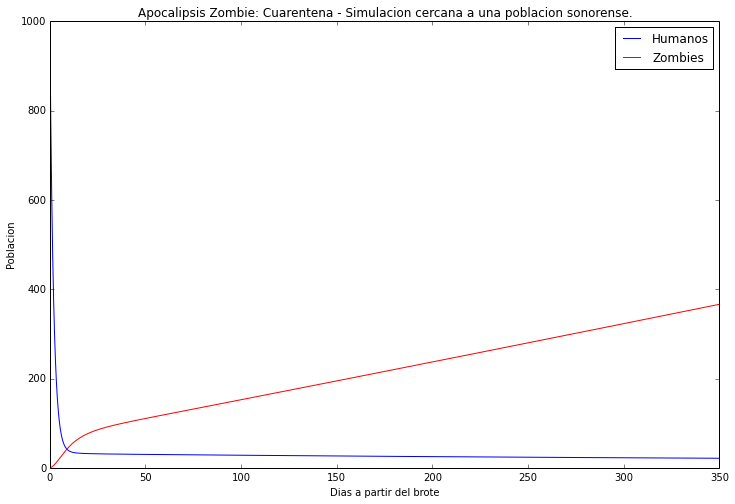
\includegraphics[scale=0.5]{sonora.png}\\

Donde podemos observar que la población humana duraría mas de un año, pero con una reducción drástica dentro de los primero 20 días, para seguir con un aumento significativo de la población de zombies. Por lo que podemos decir que un plan donde se considere solamente la cuarentena, sin eliminar inmediatamente a los zombies y sin la búsqueda de un tratamiento para los infectados la población sonorense no posee un gran esperanza de sobrevivir.


\pagebreak

\section*{\textcolor{Red}{Resultados}}
\begin{center}
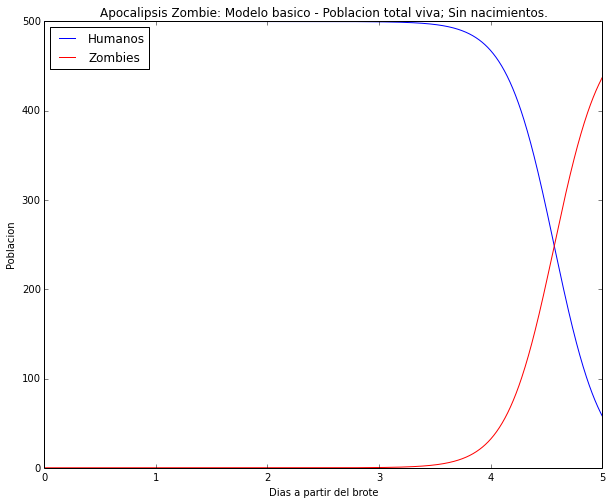
\includegraphics[scale=0.5]{act11b.png}\\
\end{center}
\begin{center}
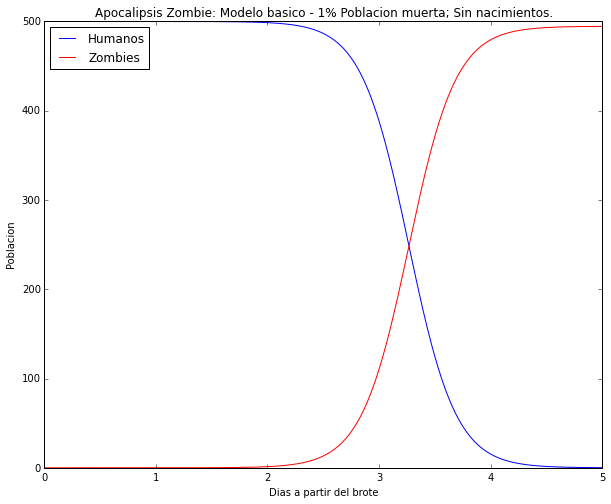
\includegraphics[scale=0.5]{act11b1.png}\\
\end{center}
\begin{center}
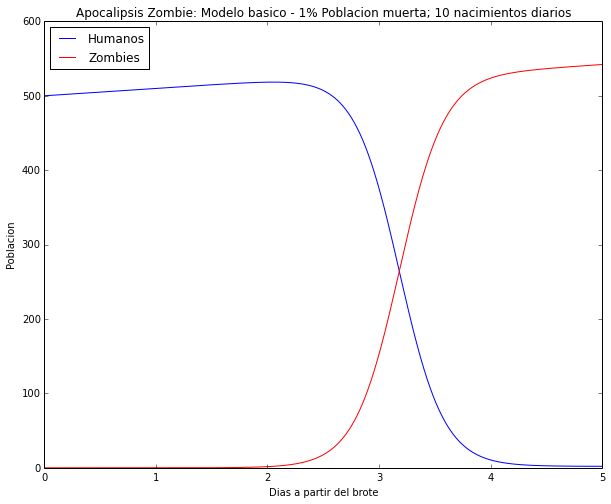
\includegraphics[scale=0.5]{act11b2.png}
\end{center}

\begin{center}
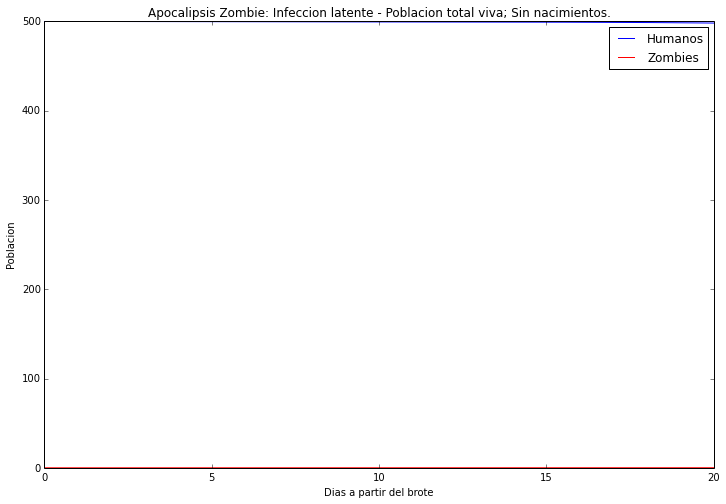
\includegraphics[scale=0.5]{act11i.png}
\end{center}

\begin{center}
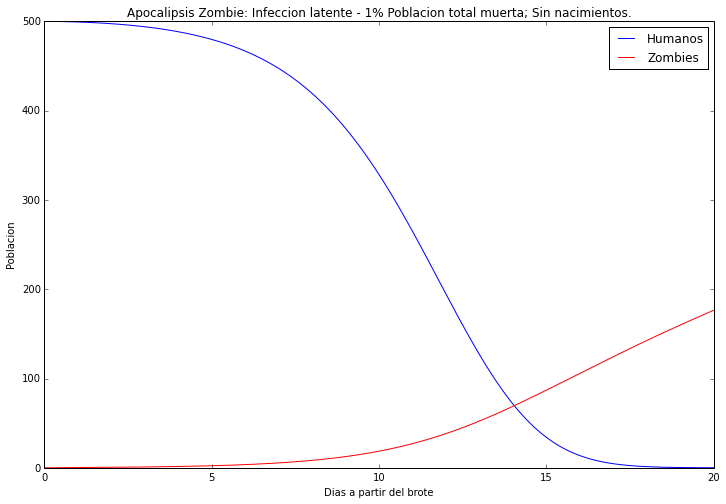
\includegraphics[scale=0.5]{act11i1.png}
\end{center}

\begin{center}
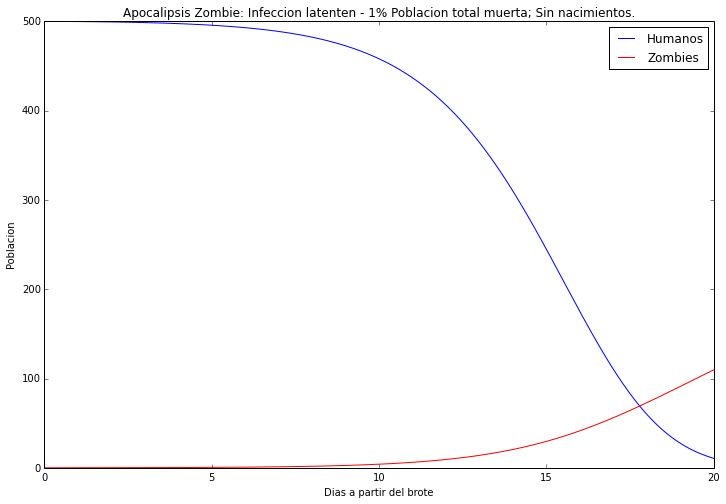
\includegraphics[scale=0.5]{act11i2.png}
\end{center}

\begin{center}
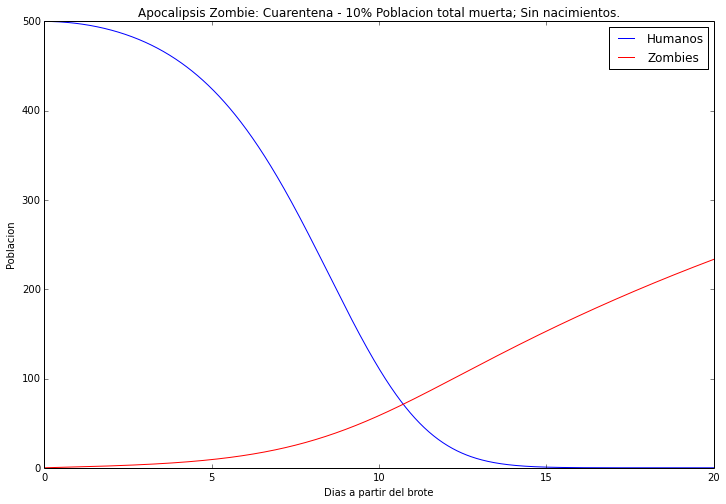
\includegraphics[scale=0.5]{act11c.png}
\end{center}

\begin{center}
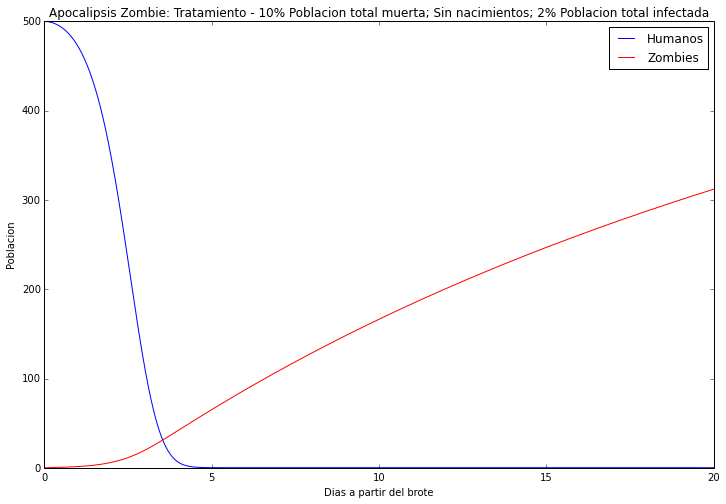
\includegraphics[scale=0.5]{act11t.png}
\end{center}
\pagebreak

\section*{\textcolor{Red}{Anexos}}

\subsection*{Modelo básico.}
\begin{boxedverbatim}
#Parámetros
P = 0       # Tasa de Natalidad
d = 0.0001  # Muertes naturales por día
B = 0.0095  # Parámetro de transmisión  (per day)
G = 0.0001  # Removidos que se convierten en zombies (per day)
A = 0.0001  # Destruidos  (per day)

# solve the system dy/dt = f(y, t)
def f(y, t):
    Si = y[0] #suceptibles a convertirse
    Zi = y[1] #Zombies
    Ri = y[2] #removidos
    # Sistema de ecuaciones
    f0 = P - B*Si*Zi - d*Si #Suceptibles
    f1 = B*Si*Zi + G*Ri - A*Si*Zi #Zombies
    f2 = d*Si + A*Si*Zi - G*Ri #Removimos
    return [f0, f1, f2]

# Condiciones Iniciales
S0 = 500.                   # Pobación humana
Z0 = 0                      # Población zombie
R0 = 0                      # Población muerta
y0 = [S0, Z0, R0]   # initial condition vector
t  = np.linspace(0, 5., 1000)       # Tiempo

\end{boxedverbatim}\\

\subsection*{Modelo con infecci\'on latente.}

\begin{boxedverbatim}
# Modelo de apocalipsis zombie: 
# Modelo con infección latente

#Parámetros
P = 0       # Tasa de Natalidad por día
d = 0.0001  # Muertes naturales por día
B = 0.0095  # Parámetro de transmisión  (per day)
G = 0.0001  # Removidos que se convierten en zombies (per day)
A = 0.0001  # Destruidos  (per day)
p = 0.05  #Parámetro de infectados
# solve the system dy/dt = f(y, t)
def f(y, t):
    Si = y[0] #suceptibles a convertirse
    Zi = y[1] #Zombies
    Ri = y[2] #Removidos
    Ii = y[3] #Infectados
    
    # Sistema de ecuaciones
    f0 = P - B*Si*Zi - d*Si #Suceptibles
    f1 = p*Ii + G*Ri - A*Si*Zi #Zombies
    f2 = d*Si + d*Ii+ A*Si*Zi - G*Ri #Removidos
    f3 = B*Si*Zi - p*Ii - d*Ii #Infectados
    return [f0, f1, f2, f3]

# Condiciones Iniciales
S0 = 500.                   # Pobación humana
I0 = 0                      # Población infectada
Z0 = 0                      # Población zombie
R0 = 0                      # Población muerta
y0 = [S0, Z0, R0, I0]   # initial condition vector
t  = np.linspace(0, 20., 1000)       # Tiempo
\end{boxedverbatim}

\subsection*{Modelo con cuarentena.}

\begin{boxedverbatim}
# Modelo de apocalipsis zombie: 
# Modelo con cuarentena

#parámetros
P = 0       # Tasa de Natalidad por día
d = 0.0001  # Muertes naturales por día
B = 0.0095  # Parámetro de transmisión  (per day)
G = 0.01  # Removidos que se convierten en zombies (per day)
A = 0.0001  # Destruidos  (per day)
p = 0.05  #Parámetro de infectados
k = 0.01  #Porcentaje de  infectados en cuarentena
s = 0.001  #Porcentage de zombies en cuarentena
n = 0.001  #Pocentaje eliminado que escapa de cuarentena
# solve the system dy/dt = f(y, t)
def f(y, t):
    Si = y[0] #suceptibles a convertirse
    Zi = y[1] #Zombies
    Ri = y[2] #Removidos
    Ii = y[3] #Infectados
    Qi = y[4] #Cuarentena
    
    # Sistema de ecuaciones
    f0 = P - B*Si*Zi - d*Si #Suceptibles
    f1 = p*Ii + G*Ri - A*Si*Zi - s*Zi #Zombies
    f2 = d*Si + d*Ii+ A*Si*Zi - G*Ri + n*Qi #Removidos
    f3 = B*Si*Zi - p*Ii - d*Ii - n*I0 #Infectados
    f4 = k*Ii + s*Zi - n*Qi #En cuarentena
    return [f0, f1, f2, f3, f4]

# Condiciones Iniciales
S0 = 500.                   # Pobación humana
I0 = 10                     # Población infectada
Z0 = 0                      # Población zombie
R0 = 50                      # Población muerta
Q0 = 0                      # Población en cuarentena
y0 = [S0, Z0, R0, I0, Q0]   # initial condition vector
t  = np.linspace(0, 20., 1000)       # Tiempo
\end{boxedverbatim}

\subsection*{Modelo con tratamiento.}

\begin{boxedverbatim}
# Modelo de apocalipsis zombie: 
# Modelo con tratamiento

#Parámetro
P = 0       # Tasa de Natalidad por día
d = 0.0001  # Muertes naturales por día
B = 0.095  # Parámetro de transmisión  (per day)
G = 0.01  # Removidos que se convierten en zombies (per day)
A = 0.0001  # Destruidos  (per day)
p = 0.005  #Parámetro de infectados
c = 0.01  #Porcentaje de zombies curados

# solve the system dy/dt = f(y, t)
def f(y, t):
    Si = y[0] #suceptibles a convertirse
    Zi = y[1] #Zombies
    Ri = y[2] #Removidos
    Ii = y[3] #Infectados
    
    # Sistema de ecuaciones
    f0 = P - B*Si*Zi - d*Si + c*Zi #Suceptibles
    f1 = p*Ii + G*Ri - A*Si*Zi - s*Zi #Zombies
    f2 = d*Si + d*Ii+ A*Si*Zi - G*Ri #Removidos
    f3 = B*Si*Zi - p*Ii - d*Ii  #Infectados

    return [f0, f1, f2, f3]

# Condiciones Iniciales
S0 = 500.                   # Pobación humana
I0 = 10                     # Población infectada
Z0 = 0                      # Población zombie
R0 = 50                      # Población removida

y0 = [S0, Z0, R0, I0]   # initial condition vector
t  = np.linspace(0, 20., 1000)       # Tiempo
\end{boxedverbatim}
\pagebreak

\begin{thebibliography}{X}
\bibitem{1} \textsc{Munz P., Hudea I., Imad J.  \& Smith R; "When zombies attack!: Mathematical modelling of an outbreak of zombie infection"}
 \bibitem{2} \textsc{Zombiepedia:"Zombies"; 2016}
 \bibitem{3} \textsc{Zombiepedia:"Types of Zombies"; 2016}
\end{thebibliography}
\end{document}